\section{User Experiment}

[Yu] The goal of the experiment is ...

The experiment has two parts. Part A is a chess game with different conditions of cues. Results support the idea of classification in our framework. Part B is the Rock-Paper-Scissors game. It requires a low delay. We present a simple assistant design to help synchronization.

The experiment is also an example. It illustrates how to measure the noticeable delay and the acceptable delay for a specific application.

\subsection{Part A: Playing Chess}

Part A was to study the variety of delay perception in different synchronization level. The task was a chess game between pairs of participants in two rooms, with two conditions of cues: audiovisual mode and visual only mode.

\subsubsection{Experimental design}

We used a within-subjects experimental design. Each pair of participants played chess in two sessions of Communication Channel (CC): \emph{audiovisual CC} and \emph{visual only CC}, which correspond to the 2nd and 3rd synchronization level. The CC conditions were assigned to participant pairs in a Latin square design. Delay was another within-subjects factor with five conditions (50, 150, 250, 450, 750 ms in \emph{audiovisual CC}; 150, 450, 1050, 1550, 2050 ms in \emph{visual only CC}). In each session, we tested the five delay conditions in five trials. The delay conditions were assigned in a random order. In particular, we encouraged participants to chat in the \emph{audiovisual CC}.

\subsubsection{Task}

In each trial, two distributed participants played chess "face-to-face" for three minutes. We adopted \emph{Reversi} as the task. \emph{Reversi} is simple enough that the participants can learn it in a short time. The game involves frequent interaction: when capturing, a participant should ask his partner to remove the captured chess. The participants have enough chances to perceive a noticeable delay.

In the physical world, each player interacted with a chessboard and chess pieces on his own side. The 3DTI system fused the two physical scenes into a virtual space. In the virtual space, each player could see not only his chess pieces but also his partner' s chess pieces.

\subsection{Part B: Rock-Paper-Scissors}

Part B was to evaluate the impact of delay in a high delay requirement situation. We used the Rock-Paper-Scissors game. We designed a synchronized audio cue to help users to synchronize with each other. The study assesses its effect on user experience.

\subsubsection{Experimental design}

This part was also a within-subjects design. Each pair played the Rock-Paper-Scissors game in two sessions: with and without the synchronized audio cue. We applied Latin square to the two sessions. In each session, we tested the delay of 50, 83, 117 and 150ms in four trials. The order of delay conditions was random. We also adopted Latin square on part A and part B.

\subsubsection{Task}

In each trial, a pair continuously drew the Rock-Paper-Scissors gestures until one of them won for ten times. There were two conditions to test: with and without the synchronized visual cue. In an actual network, it is possible to synchronize the time of two systems with almost zero milliseconds apart (the NTP protocol [?]).

Our 3DTI system provided zero-delay audio cues for both users to help them gesture exactly at the same time. The cue was an audio source of four seconds, with "tick" sounds at the 2nd, 3rd second and a "tack" sound at the 4th second. We told participants to gesture when their hear the "tack" sound.

\subsection{Participants}

We advertised our experiment on social media. Sixteen pairs of participants took part in our experiment (32 in total, xx females). They all came from the campus, aged from xx to xx. Participants were paid 150 yuan for the 90 minutes long study. The ten participants with the most conversation turn received extra 50 yuan.

Previous works have pointed out that the individual user differences affect study results of delay perception [?]. In our experiment, we control the source of participants carefully:

\begin{itemize}
    \item \emph{Relationship}: Each pair of participants are familiar with each other (friends, classmates or partners). This setting is to improve the conversation quality.
    
    \item \emph{First language}: All the participants are native Chinese speakers. Chinese conversations are a little bit harder to predict compared to English conversations [?], which may lead to a larger noticeable delay (about xx ms).
    
    \item \emph{Experience in DIME}: Our participants have relatively high education levels. According to the self-report questionnaire, they are quite familiar with audiovisual multimedia (xx points in average, 5 for experts) and AR/VR (xx points in average).
\end{itemize}

Thus, our study results are rigorous but relatively low in the external validity. We recommend a larger amount of participants if the readers need a more general result.

\subsection{Procedure}

%[Copy from other paper] Each pair of participants completed consent forms at the study location. They were then taken to separate study rooms containing the audiovisual telecommunications stations. The experimenters informed the participants that they would have seven 4-minute conversations using the stations, and that they would be given topic sheets for inspiration. Participants could use a small timer to keep track of their conversation, and they were informed that the experimenter would interrupt the conversation once four minutes had passed. Once seated, participants were given headphones and the first topic sheet. Participants were told to start whenever they both were ready. The experimenters then left the study rooms to monitor the conversations from a nearby location.

%[Copy from other paper] After four minutes, the experimenters interrupted the conversations, gave the participants short surveys to complete, and presented the next topic sheet. This process was repeated for each of the seven trials. After all seven trials, participants completed a questionnaire asking about their favorite conversations and any difficulties with understanding the other participant.

Before the experiment, we invited the participant pair to a room and explained our study. We explained the rule of \emph{Reversi} and \emph{Rock-Paper-Scissors}. Next, the pair had ten minutes to experience the physical interaction of these two games. We asked the participants to remember the feeling of physical interaction and regard it as a zero-delay experience. Then, we introduced our experimental procedure to the participants.

Part A had $2 sessions \times 5 trials = 10 trials$, which lasted for 40 minutes. Part B had $2 sessions \times 4 trials = 8 trials$ (20 minutes). In each trial, the participants experience the remote VR game. After each trial, participants filled in a short survey and rested for one minute. The questions in the survey are shown in Table \ref{tab:table_experiment}.

\begin{table} [!htbp]
\begin{tabular}{|p{0.25\columnwidth}|p{0.35\columnwidth}|p{0.3\columnwidth}|}
\hline 
Label & Question & Scale \\
\hline
quality & How do you feel during the experiment? & Bad <--> Excellent \\
\hline
noticeability & Can you perceive the delay in the connection? & Very much <--> Not at all \\
\hline
tolerance & To what extent where you annoyed by the delay? & Severe annoyance <--> No annoyance \\
\hline
\end{tabular}
\caption{Questions and scale.}
\label{tab:table_experiment}
\end{table}

After each session, participants had a five minutes break. We conducted brief interviews with some subjective questions as followed:

\begin{itemize}
    \item How do you notice the delay? What are the cues?
    
    \item What makes you annoyed in the task?
    
    \item Any other comments?
\end{itemize}

In particular, we explained to participants about the concept of network delay. In our system, there was a local end-to-end delay of about 20 ms, which is slightly noticeable for the users. We told the participants that we do not consider the local delay in the questionnaire. Instead, we evaluate the network delay, which is the time interval between your partner acts and you see. A participant can perceive the network delay by judging if his partner is slow in speaking and gesturing.

\subsection{Results}


[NOTE from zsyzgu] I have several ideas about the result:

\begin{itemize}
    \item In 3DTI, the users are much more tolerable than in audiovisual DIME. The immersive environment makes users focus on the interaction itself.
    \item A simple synchronized audio cue can help synchronization in tasks with high network requirement.
    \item Conversation is a stronger cue compared with visual feedback.
    \item Delay perception of 50 ms and 150 ms in audiovisual model have no significant difference.
    \item The individual user differences are larger in 3DTI.
\end{itemize}


\subsubsection{Delay Effects}[TODO]

Attention: Analysis from only 6 groups of data.

\begin{figure}[H]
\centering
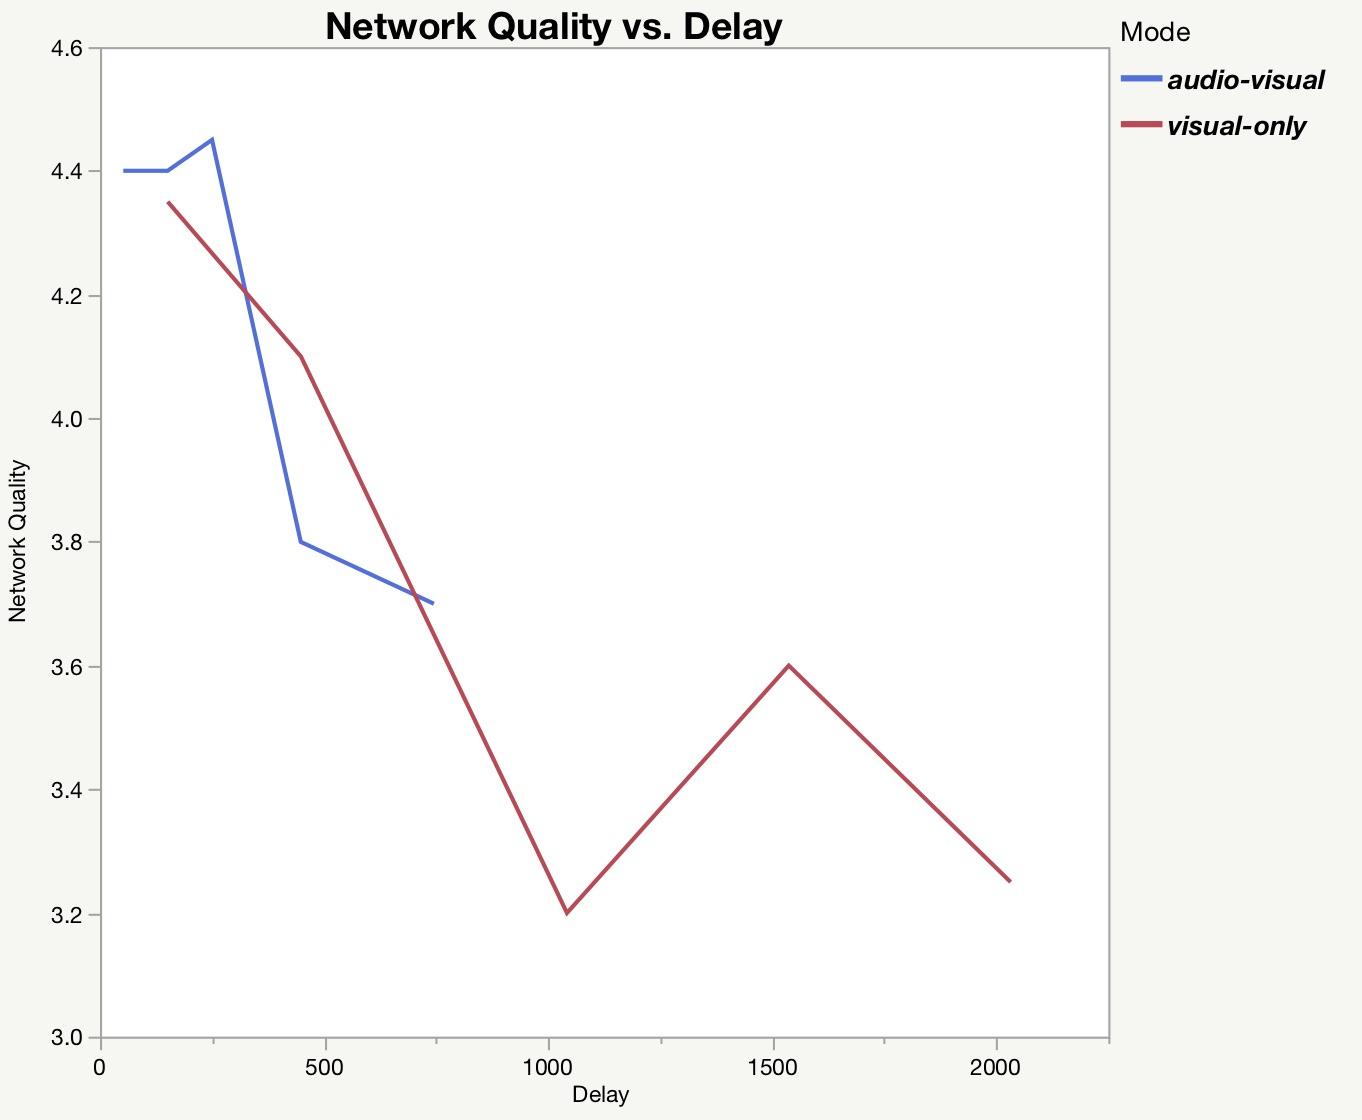
\includegraphics[width=6cm]{figures/figure_experiment1_NQ.jpg}
\setlength{\abovecaptionskip}{0.5cm}
\caption{Effects of delay on quality score in part A(Playing Chess).}
\label{4}
\end{figure}

\begin{figure}[H]
\centering
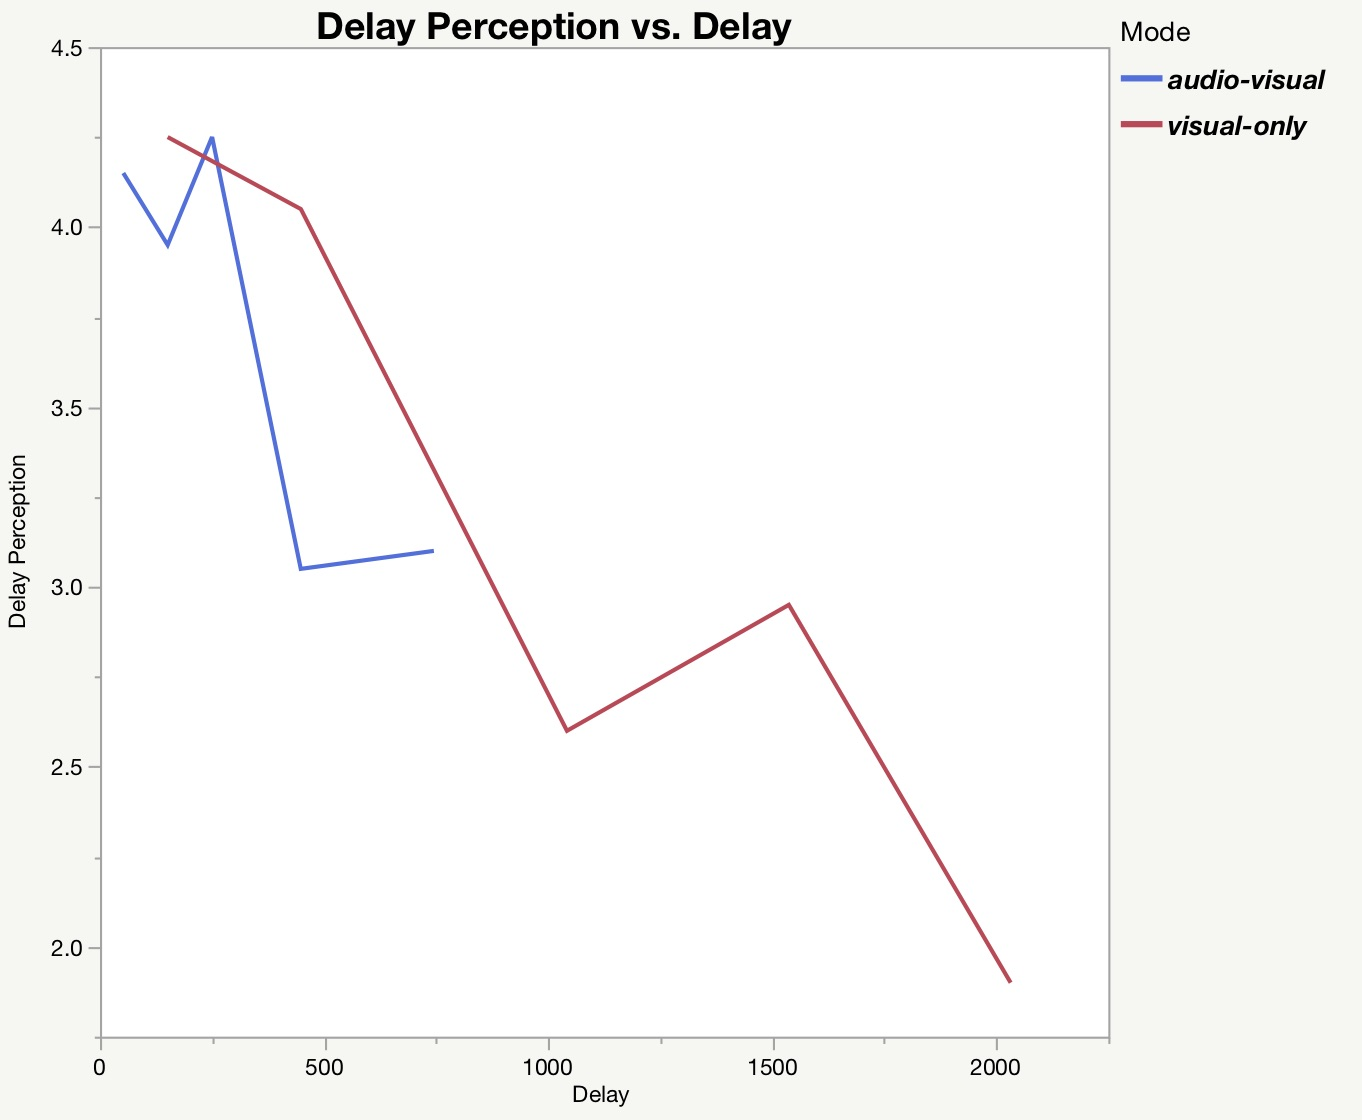
\includegraphics[width=6cm]{figures/figure_experiment1_DP.jpg}
\setlength{\abovecaptionskip}{0.5cm}
\caption{Effects of delay on noticeability score in part A(Playing Chess).}
\label{4}
\end{figure}

\begin{figure}[H]
\centering
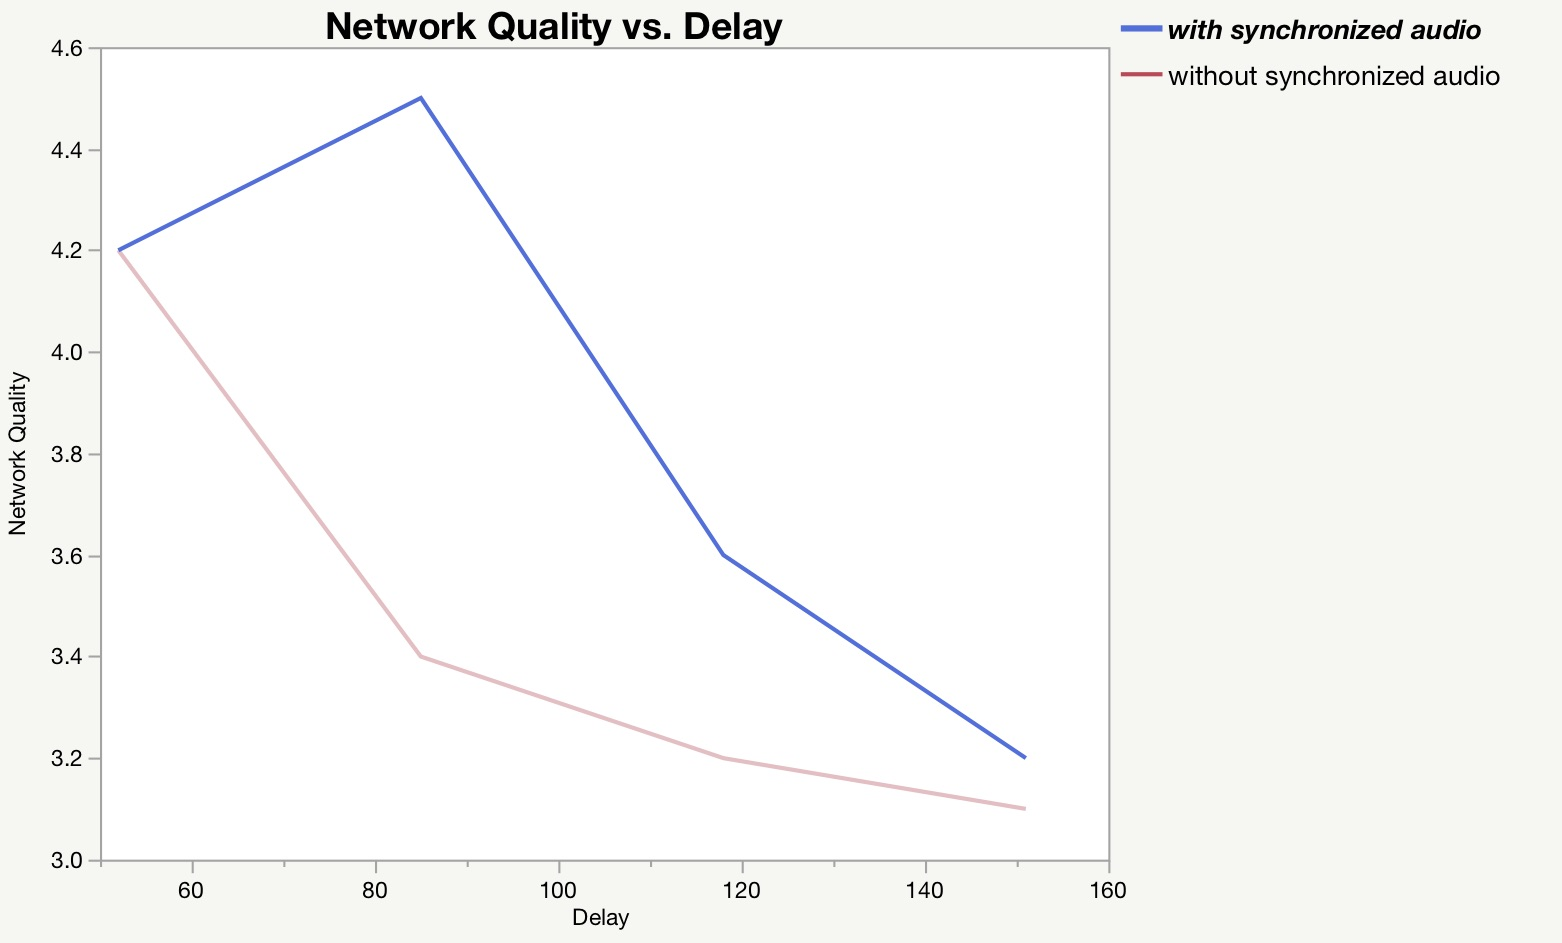
\includegraphics[width=6.9cm]{figures/figure_experiment2_NQ.jpg}
\setlength{\abovecaptionskip}{0.5cm}
\caption{Effects of delay on quality score in part B(Rock-Paper-Scissors).}
\label{4}
\end{figure}

\begin{figure}[H]
\centering
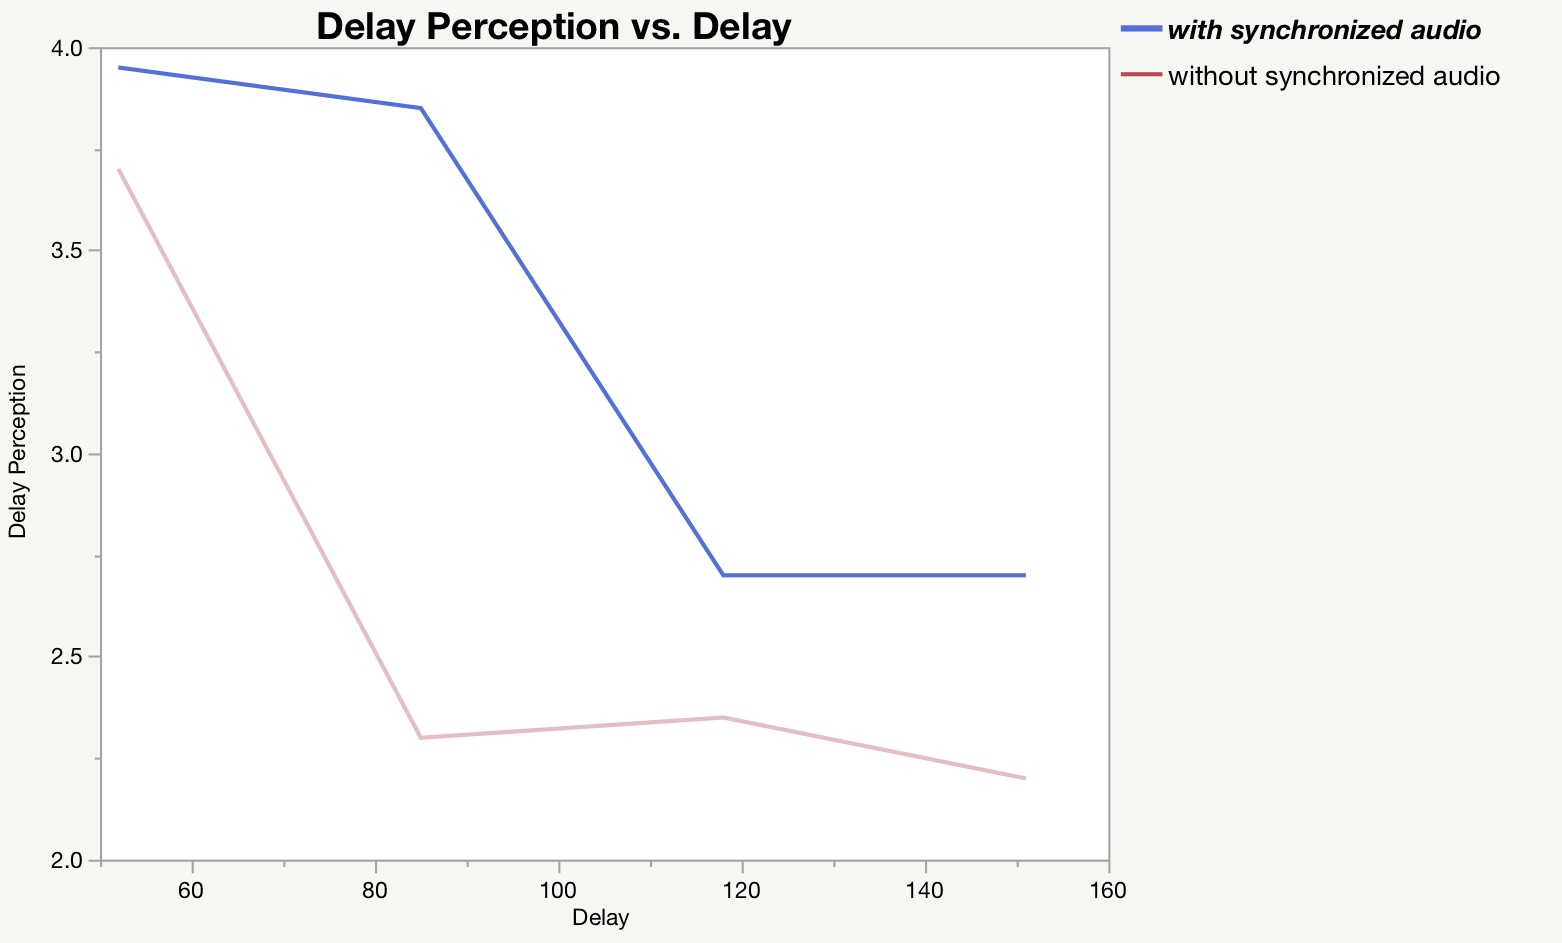
\includegraphics[width=6.9cm]{figures/figure_experiment2_DP.jpg}
\setlength{\abovecaptionskip}{0.5cm}
\caption{Effects of delay on noticeability score in part B(Rock-Paper-Scissors).}
\label{4}
\end{figure}


\subsubsection{Data Analysis}[TODO]

\begin{table} [!htbp]
\begin{tabular}{|p{0.3\columnwidth}|p{0.15\columnwidth}|p{0.3\columnwidth}|p{0.15\columnwidth}|}
\hline 
Difference & 0.30000 & t Radio & 0.582772 \\
\hline
Std Err Dif & 0.5148 & DF & 15.92888 \\
\hline
Upper CL Dif & 1.3917 & Prob > |t| & 0.5682 \\
\hline
Lower CL Dif & -0.7917 & Prob > t & 0.2841 \\
\hline
Confidence & 0.95 & Prob < t & 0.7159 \\
\hline
\end{tabular}
\caption{Oneway analysis of noticeability score by mode(Delay = 150ms)}
\label{tab:table_questionnaire}
\end{table}


\begin{table} [!htbp]
\begin{tabular}{|p{0.3\columnwidth}|p{0.15\columnwidth}|p{0.3\columnwidth}|p{0.15\columnwidth}|}
\hline 
Difference & 1.0000 & t Radio & 1.678363 \\
\hline
Std Err Dif & 0.5958 & DF & 14.9258 \\
\hline
Upper CL Dif & 2.2705 & Prob > |t| & 0.1141 \\
\hline
Lower CL Dif & -0.2705 & Prob > t & 0.0570 \\
\hline
Confidence & 0.95 & Prob < t & 0.9430 \\
\hline
\end{tabular}
\caption{Oneway analysis of noticeability score by mode(Delay = 450ms)}
\label{tab:table_questionnaire}
\end{table}
